\documentclass[11pt,a4paper]{article}

\usepackage[T1]{fontenc}
\usepackage[utf8]{inputenc}
\frenchspacing
\usepackage{amsmath,amssymb,amsthm,mathtools}
\usepackage[margin=2.5cm]{geometry}
\usepackage{tikz}
\usepackage{pgfplots}
\pgfplotsset{compat=1.16}
\usepackage{array}
\usepackage{booktabs}
\usepackage{xcolor}
\usepackage[most]{tcolorbox}
\usepackage{enumitem}
\usepackage{hyperref}
\hypersetup{colorlinks=true,linkcolor=black,citecolor=black,urlcolor=blue!55!black}

% ---------- Parties en français ----------
\renewcommand{\partname}{Partie}

% ---------- Environnements (partagés par les deux parties) ----------
\theoremstyle{plain}
\newtheorem{theoreme}{Théorème}
\newtheorem{lemme}{Lemme}
\newtheorem{proposition}{Proposition}
\newtheorem{corollaire}{Corollaire}
\theoremstyle{definition}
\newtheorem{definition}{Définition}
\newtheorem{remarque}{Remarque}
\newtheorem{exemple}{Exemple}

% ---------- Notations ----------
\newcommand{\R}{\mathbb{R}}
\newcommand{\N}{\mathbb{N}}
\newcommand{\A}{\mathcal{A}}
\newcommand{\1}{\mathbf{1}}
\newcommand{\ind}[1]{\1_{#1}}
\newcommand{\abs}[1]{\left|#1\right|}
\newcommand{\norm}[1]{\left\lVert#1\right\rVert}
\newcommand{\pp}{\text{p.p.}}
\DeclareMathOperator{\intt}{int}
\DeclareMathOperator*{\esssup}{ess\,sup}

% ---------- Encadré dualité ----------
\newtcolorbox{boitedual}{
  enhanced, colback=orange!5, colframe=orange!55!black,
  boxrule=0.6pt, arc=2pt, left=8pt, right=8pt, top=6pt, bottom=6pt,
  title=\textbf{La dualité mesure/catégorie et ses limites},
  fonttitle=\bfseries, coltitle=black, colbacktitle=orange!18,
  attach boxed title to top left={xshift=8pt,yshift=-2mm},
  boxed title style={colframe=orange!55!black,boxrule=0.5pt,arc=1pt}
}

\title{\bfseries De la convergence presque partout à la catégorie\\[0.35em]
\large Egorov et Osgood : un même argument de recouvrement, deux notions de « petit »}
\author{}
\date{}

\begin{document}
\maketitle
\vspace{-2.0em}

\begin{center}
\begin{minipage}{0.9\textwidth}\small
\noindent\textbf{Résumé.} La \textbf{Partie~I} établit le théorème d'Egorov : sur
un espace de mesure finie, la convergence presque partout d'une suite de fonctions
mesurables devient uniforme en dehors d'un ensemble de mesure arbitrairement
petite. La démonstration est détaillée sous forme de deux lemmes — dont l'un isole
le rôle de la finitude — puis complétée par deux contre-exemples (optimalité des
hypothèses) et par la variante \emph{dominée}, valable sans finitude globale. La
\textbf{Partie~II} dégage l'analogue topologique : le théorème d'Osgood (limite
simple de fonctions continues $\Rightarrow$ convergence localement uniforme sur un
$G_\delta$ dense) repose sur \emph{exactement le même squelette}, le théorème de
Baire y jouant le rôle de la continuité de la mesure. On met les deux
démonstrations en vis-à-vis, on rattache le mécanisme au théorème de
Banach--Steinhaus, et l'on précise le statut \emph{heuristique} de la dualité
mesure/catégorie d'Oxtoby.
\end{minipage}
\end{center}
\vspace{0.4em}

{\small\tableofcontents}
\bigskip

% =====================================================================
\part{Le théorème d'Egorov}
% =====================================================================

\section{Énoncé}

Dans tout ce qui suit, $(X,\A,\mu)$ désigne un espace mesuré et les fonctions
considérées sont mesurables, à valeurs dans $\R$ ou $\mathbb{C}$.

\begin{definition}
On dit que $(f_n)$ converge \emph{presque uniformément} vers $f$ si, pour tout
$\varepsilon>0$, il existe $A\in\A$ tel que $\mu(X\setminus A)<\varepsilon$ et
$f_n\to f$ uniformément sur $A$.
\end{definition}

\begin{theoreme}[Egorov, 1911]\label{th:egorov}
Soit $(X,\A,\mu)$ un espace mesuré \textbf{de mesure finie}, $\mu(X)<\infty$.
Soit $(f_n)$ une suite de fonctions mesurables convergeant $\mu$-presque partout
vers une fonction $f$. Alors $(f_n)$ converge presque uniformément vers $f$.
\end{theoreme}

\paragraph{L'idée.} La convergence presque partout est \emph{ponctuelle} : le rang
à partir duquel $\abs{f_m(x)-f(x)}$ devient petit dépend du point $x$, et rien
n'interdit a priori que ce rang explose lorsque $x$ parcourt $X$. Egorov affirme
que ce phénomène de « rangs qui divergent » ne peut se concentrer que sur un
ensemble de mesure petite : on l'excise, et sur le reste la convergence redevient
uniforme. La finitude de $\mu$ est l'unique ingrédient empêchant que la
« mauvaise » masse ne s'échappe à l'infini.

\section{Démonstration}\label{sec:preuve-egorov}

Quitte à retirer un ensemble négligeable, on suppose la convergence \textbf{en tout
point} de $X$ : cela ne modifie ni $f$, ni la mesure des ensembles introduits
ci-dessous. Pour $n,k\ge 1$, posons
\[
  E_{n,k}\;=\;\bigcup_{m\ge n}\Bigl\{\,x\in X:\ \abs{f_m(x)-f(x)}\ge\tfrac1k\,\Bigr\}.
\]
Intuitivement, $E_{n,k}$ est l'ensemble des points qui, \emph{au-delà} du rang $n$,
ratent au moins une fois la précision $1/k$.

\begin{lemme}[Décroissance et intersection vide]\label{lem:decr}
À $k$ fixé, la suite $(E_{n,k})_{n\ge1}$ est décroissante et
$\displaystyle\bigcap_{n\ge1}E_{n,k}=\varnothing$.
\end{lemme}

\begin{proof}
La décroissance est immédiate : passer de $n$ à $n+1$ retire des termes de la
réunion, donc $E_{n+1,k}\subseteq E_{n,k}$. Ensuite,
\[
  \bigcap_{n\ge1}E_{n,k}
  =\Bigl\{\,x:\ \abs{f_m(x)-f(x)}\ge\tfrac1k\ \text{pour une infinité de }m\,\Bigr\}.
\]
En effet, $x$ appartient à cette intersection si et seulement si, pour tout $n$,
il existe $m\ge n$ avec $\abs{f_m(x)-f(x)}\ge 1/k$, ce qui est exactement dire que
l'inégalité a lieu pour une infinité d'indices. Or, pour chaque $x$ fixé, la
convergence $f_m(x)\to f(x)$ entraîne $\abs{f_m(x)-f(x)}<1/k$ pour tout $m$ assez
grand : l'inégalité $\ge 1/k$ n'a lieu que pour un nombre \emph{fini} d'indices.
L'intersection est donc vide.
\end{proof}

\begin{lemme}[Le rôle de la finitude]\label{lem:fini}
Si $\mu(X)<\infty$, alors pour tout $k\ge1$,
$\displaystyle\lim_{n\to\infty}\mu(E_{n,k})=0$.
\end{lemme}

\begin{proof}
Comme $\mu(X)<\infty$, on a en particulier $\mu(E_{1,k})<\infty$. La suite
$(E_{n,k})_n$ décroît vers l'ensemble vide (Lemme~\ref{lem:decr}), donc la
\emph{continuité de la mesure par le haut} — valable précisément parce que le
premier terme est de mesure finie — donne
\[
  \lim_{n\to\infty}\mu(E_{n,k})
  =\mu\Bigl(\bigcap_{n\ge1}E_{n,k}\Bigr)
  =\mu(\varnothing)=0. \qedhere
\]
\end{proof}

\begin{proof}[Démonstration du Théorème~\ref{th:egorov}]
Fixons $\varepsilon>0$. Pour chaque $k\ge1$, le Lemme~\ref{lem:fini} fournit un
rang $n_k$ tel que
\[
  \mu\bigl(E_{n_k,\,k}\bigr)<\frac{\varepsilon}{2^{\,k}}.
\]
Posons
\[
  A\;=\;X\setminus\bigcup_{k\ge1}E_{n_k,\,k},
  \qquad\text{de sorte que}\qquad
  A^{c}=\bigcup_{k\ge1}E_{n_k,\,k}.
\]

\emph{Mesure du complémentaire.} Par sous-additivité dénombrable,
\[
  \mu(A^{c})\;\le\;\sum_{k\ge1}\mu\bigl(E_{n_k,\,k}\bigr)
  \;<\;\sum_{k\ge1}\frac{\varepsilon}{2^{\,k}}\;=\;\varepsilon.
\]

\emph{Convergence uniforme sur $A$.} Soit $x\in A$. Alors $x\notin E_{n_k,k}$ pour
\emph{tout} $k$. Par définition de $E_{n_k,k}$, cela signifie exactement
\[
  \forall k\ge1,\ \forall m\ge n_k,\qquad \abs{f_m(x)-f(x)}<\tfrac1k .
\]
Soit $\delta>0$. Choisissons $k$ tel que $1/k<\delta$. Alors, pour tout $m\ge n_k$
et pour tout $x\in A$ \emph{simultanément},
\[
  \abs{f_m(x)-f(x)}<\tfrac1k<\delta .
\]
Le rang $n_k$ ne dépend pas de $x$ : c'est la définition même de la convergence
uniforme de $(f_n)$ vers $f$ sur $A$.
\end{proof}

\section{Optimalité des hypothèses}

\subsection*{La finitude est indispensable}

\begin{exemple}\label{ex:masse}
Sur $(\R,\mathcal{B}(\R),\lambda)$, posons $f_n=\ind{[n,\,n+1]}$. Alors $f_n\to 0$
en tout point (chaque $x$ n'est couvert que par un nombre fini de $f_n$).
Pourtant, pour tout ensemble $A$ dont le complémentaire est de mesure finie, il
existe une infinité d'indices $n$ tels que $A\cap[n,n+1]$ soit de mesure
strictement positive, donc $\sup_A\abs{f_n}=1$ pour ces indices : aucune
convergence uniforme sur $A$ n'est possible. La masse s'échappe vers l'infini et
la continuité par le haut du Lemme~\ref{lem:fini} s'effondre ($\mu(E_{n,1})=+\infty$
pour tout $n$).
\end{exemple}

\paragraph{Pourquoi la finitude ?} La phrase « la continuité par le haut
s'effondre » mérite d'être disséquée : on va localiser l'endroit \emph{exact} où la
finitude entre en jeu, puis vérifier que l'exemple ci-dessus retombe mot pour mot
sur le contre-exemple canonique.

\begin{proposition}[Continuité par le haut, et sa dépendance à la finitude]
\label{prop:contHaut}
Soit $(A_n)_{n\ge1}$ une suite \emph{décroissante} de $\A$, $A_n\downarrow A
=\bigcap_n A_n$. \textbf{Si} l'un des termes est de mesure finie --- disons
$\mu(A_1)<\infty$ --- alors $\mu(A_n)\to\mu(A)$. Cette hypothèse de finitude est
indispensable.
\end{proposition}

\begin{proof}
On se ramène à la continuité par le \emph{bas}, qui, elle, est
\textbf{inconditionnelle} : pour toute suite croissante $B_n\uparrow B$, la
$\sigma$-additivité appliquée à la partition
$B=B_1\sqcup\bigsqcup_{n\ge1}(B_{n+1}\setminus B_n)$ donne
$\mu(B_n)\uparrow\mu(B)$, sans aucune restriction de finitude.

Posons $B_n=A_1\setminus A_n$. Comme $(A_n)$ décroît, $(B_n)$ croît, et
$B_n\uparrow A_1\setminus A$ ; la continuité par le bas fournit donc
$\mu(A_1\setminus A_n)\to\mu(A_1\setminus A)$. \emph{C'est ici, et seulement ici,
qu'intervient la finitude} : puisque $A_n\subseteq A_1$ et $A\subseteq A_1$ avec
$\mu(A_1)<\infty$, on a le droit d'écrire
\[
  \mu(A_1\setminus A_n)=\mu(A_1)-\mu(A_n),\qquad
  \mu(A_1\setminus A)=\mu(A_1)-\mu(A),
\]
l'identité $\mu(B\setminus C)=\mu(B)-\mu(C)$ (pour $C\subseteq B$) n'étant licite
que si $\mu(C)<\infty$, ce qui est ici garanti car $\mu(A_n),\mu(A)\le\mu(A_1)
<\infty$. En reportant, $\mu(A_1)-\mu(A_n)\to\mu(A_1)-\mu(A)$, et en
\emph{soustrayant} le nombre fini $\mu(A_1)$ de part et d'autre, $\mu(A_n)\to\mu(A)$.

Si au contraire $\mu(A_1)=\infty$, cette dernière soustraction devient
$\infty-\infty$, forme indéterminée : le raisonnement s'arrête net. Ce n'est pas un
simple défaut de preuve, comme le montre le contre-exemple suivant.
\end{proof}

\begin{exemple}[Le contre-exemple minimal]\label{ex:minimal}
Sur $(\R,\lambda)$, prenons $A_n=[n,+\infty)$. La suite décroît vers
$\bigcap_{n\ge1}[n,+\infty)=\varnothing$, donc
$\mu\bigl(\bigcap_n A_n\bigr)=0$. Pourtant $\mu(A_n)=+\infty$ pour tout $n$, si bien
que
\[
  \lim_{n\to\infty}\mu(A_n)=+\infty\;\ne\;0=\mu\Bigl(\bigcap_{n\ge1}A_n\Bigr).
\]
La continuité par le haut est violée de la façon la plus brutale qui soit : les
mesures restent \emph{infinies} tandis que l'intersection est \emph{vide}.
\end{exemple}

\paragraph{L'exemple d'Egorov \emph{est} ce contre-exemple.} Reprenons
$f_n=\ind{[n,n+1]}$ et la précision $1/k=1$. L'ensemble des points ratant cette
précision au rang $m$ est $\{\,\abs{f_m-0}\ge1\,\}=[m,m+1]$, donc
\[
  E_{n,1}=\bigcup_{m\ge n}\{\abs{f_m}\ge1\}=\bigcup_{m\ge n}[m,m+1]=[n,+\infty).
\]
On retombe \emph{littéralement} sur l'Exemple~\ref{ex:minimal} :
$E_{n,1}\downarrow\varnothing$ mais $\mu(E_{n,1})=+\infty$ pour tout $n$. Le moteur
même de la preuve d'Egorov --- « $\mu(E_{n,k})\to0$ quand $n\to\infty$ »
(Lemme~\ref{lem:fini}) --- ne démarre jamais, faute d'un premier terme de mesure
finie.

\paragraph{L'image à retenir.} La continuité par le haut affirme qu'en rétrécissant
une famille décroissante jusqu'à son intersection, la mesure \emph{s'écoule}
progressivement vers $\mu(A)$. Encore faut-il un \emph{réservoir fini} : la masse
n'a alors nulle part où se cacher et finit forcément par s'évacuer. En mesure
infinie, la famille peut au contraire garder à chaque étape une part constante ---
voire infinie --- de masse tout en décroissant ponctuellement vers le vide : la
masse ne s'évacue pas, elle \emph{glisse vers l'infini}. À chaque pas
$[n,+\infty)\rightsquigarrow[n+1,+\infty)$, on n'abandonne qu'une tranche
\emph{finie} $[n,n+1)$, mais ce qui reste est encore de mesure infinie --- on ne
vide jamais le réservoir. C'est précisément cette fuite à l'infini que la finitude
$\mu(X)<\infty$ interdit, et c'est tout ce dont Egorov a besoin.

\subsection*{On ne peut pas prendre $\varepsilon=0$}

Le théorème produit un ensemble de complémentaire \emph{petit}, jamais
\emph{négligeable}. L'exemple canonique est $f_n(x)=x^{n}$ sur $[0,1]$, qui converge
simplement vers $\ind{\{1\}}$, soit $0$ presque partout.

\begin{center}
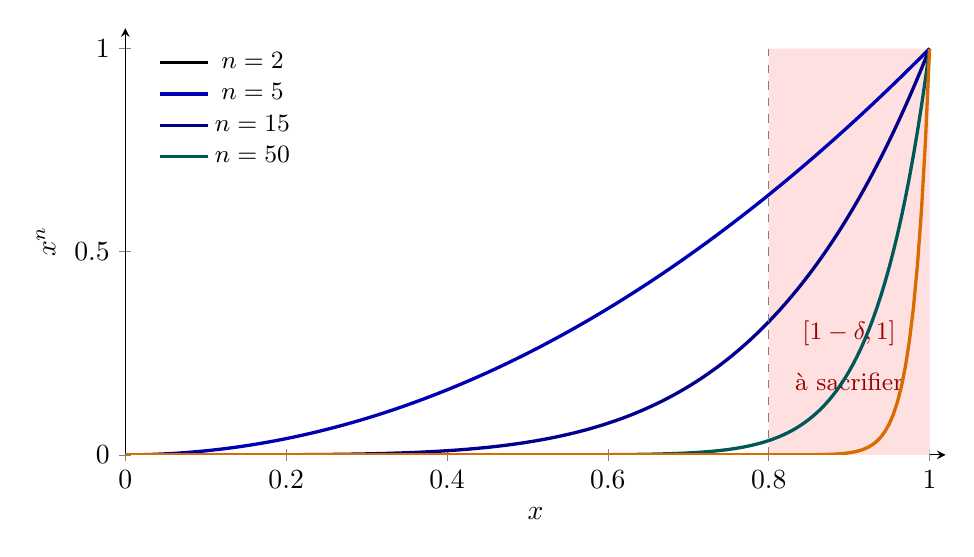
\begin{tikzpicture}
\begin{axis}[
    width=12cm, height=7cm,
    domain=0:1, samples=200,
    xmin=0, xmax=1.02, ymin=0, ymax=1.05,
    xlabel={$x$}, ylabel={$x^n$},
    axis lines=left,
    xtick={0,0.2,0.4,0.6,0.8,1},
    ytick={0,0.5,1},
    legend pos=north west,
    legend style={draw=none,fill=none,font=\small},
    every axis plot/.append style={very thick},
]
\addplot[draw=none,fill=red!12,domain=0.8:1] {1} \closedcycle;
\node[red!60!black,font=\small] at (axis cs:0.9,0.30) {$[1-\delta,1]$};
\node[red!60!black,font=\small] at (axis cs:0.9,0.18) {à sacrifier};

\addplot[blue!70!black] {x^2};   \addlegendentry{$n=2$}
\addplot[blue!55!black] {x^5};   \addlegendentry{$n=5$}
\addplot[teal!70!black] {x^15};  \addlegendentry{$n=15$}
\addplot[orange!85!black] {x^50};\addlegendentry{$n=50$}

\draw[dashed,gray] (axis cs:0.8,0) -- (axis cs:0.8,1);
\end{axis}
\end{tikzpicture}
\end{center}

\begin{exemple}\label{ex:xn}
Pour la suite $f_n(x)=x^n$ sur $[0,1]$ :
\begin{itemize}[nosep]
\item sur chaque $[0,1-\delta]$ on a $\sup_{x\le 1-\delta}x^n=(1-\delta)^n\to0$ :
      la convergence \emph{est} uniforme ;
\item mais sur $[0,1)$ privé de tout négligeable, $\sup x^n=1$ pour tout $n$ :
      jamais uniforme.
\end{itemize}
Il faut donc sacrifier un voisinage $[1-\delta,1]$ de $1$, de mesure $\delta>0$.
C'est exactement ce voisinage — de mesure aussi petite que l'on veut mais non
nulle — que fournit Egorov. On voit sur la figure que la « marche » des courbes
se resserre contre $x=1$ : la non-uniformité vit dans une couche limite de mesure
strictement positive. \emph{(Cet exemple reparaîtra en Partie~II, où sa
non-uniformité se lira au seul point $x=1$, un fermé d'intérieur vide.)}
\end{exemple}

\section{La variante dominée (sans finitude globale)}

L'inspection de la démonstration révèle que l'on n'a jamais utilisé $\mu(X)<\infty$
pour lui-même, mais uniquement la finitude de $\mu(E_{1,k})$, seule nécessaire à la
continuité par le haut du Lemme~\ref{lem:fini}. On peut donc affaiblir l'hypothèse.

\begin{theoreme}[Egorov dominé]\label{th:domine}
Soit $(X,\A,\mu)$ un espace mesuré \emph{quelconque}. Soit $(f_n)$ une suite
mesurable convergeant presque partout vers $f$. On suppose qu'il existe
$g\in L^1(\mu)$ telle que
\[
  \abs{f_n-f}\le g\quad\pp,\qquad\text{pour tout }n.
\]
Alors $(f_n)$ converge presque uniformément vers $f$.
\end{theoreme}

\begin{proof}
On reprend les ensembles $E_{n,k}$. Pour tout $m$, l'hypothèse de domination donne
$\{\abs{f_m-f}\ge 1/k\}\subseteq\{g\ge 1/k\}$, d'où
\[
  E_{n,k}\subseteq E_{1,k}\subseteq\Bigl\{g\ge\tfrac1k\Bigr\}.
\]
Par l'inégalité de Markov,
\[
  \mu\Bigl(\Bigl\{g\ge\tfrac1k\Bigr\}\Bigr)\le k\,\lVert g\rVert_{1}<\infty,
\]
donc $\mu(E_{1,k})<\infty$. Le Lemme~\ref{lem:decr} reste valable tel quel
(il n'utilise pas la mesure), et la continuité par le haut s'applique de nouveau :
$\mu(E_{n,k})\to0$ quand $n\to\infty$. Le procédé diagonal de la
Section~\ref{sec:preuve-egorov} se déroule alors à l'identique.
\end{proof}

\begin{remarque}
Cette variante éclaire le contre-exemple~\ref{ex:masse} : dominer
$f_n=\ind{[n,n+1]}$ imposerait $g\ge\ind{[1,\infty)}$, qui n'est pas intégrable.
L'absence de fonction dominante intégrable est précisément l'obstruction, et non
la $\sigma$-finitude de $\R$ (qui, elle, est bien vérifiée). La bonne hypothèse
n'est donc pas « $X$ est $\sigma$-fini » mais « la queue de la suite vit, à
précision $1/k$ fixée, sur un ensemble de mesure finie ».
\end{remarque}

\section{Les principes de Littlewood, et le théorème de Lusin}

\subsection*{Place dans la hiérarchie des convergences}

Egorov établit, en mesure finie (ou sous domination), l'implication
\[
  \text{convergence \pp}\ \Longrightarrow\ \text{convergence presque uniforme}
  \ \Longrightarrow\ \text{convergence en mesure}.
\]
La seconde implication est élémentaire : si $\mu(X\setminus A)<\varepsilon$ et la
convergence est uniforme sur $A$, alors $\mu(\{\abs{f_n-f}\ge\eta\})\le\varepsilon$
pour $n$ assez grand, et ce pour tout $\eta>0$.

\subsection*{Les trois principes de Littlewood}

Littlewood résumait la théorie de la mesure sur $\R$ par trois énoncés informels,
tous de la forme \emph{« tout objet mesurable est \textbf{presque} un objet
régulier »}, où « presque » signifie \emph{hors d'un ensemble de mesure aussi petite
que voulue} :
\begin{enumerate}[label=(\textbf{L\arabic*}),leftmargin=2.4em,itemsep=2pt,topsep=3pt]
\item tout ensemble mesurable de mesure finie est presque une réunion finie
      d'intervalles (régularité) ;
\item toute fonction mesurable est presque continue \emph{(Lusin)} ;
\item toute suite de fonctions mesurables convergeant p.p. est presque
      uniformément convergente \emph{(Egorov)}.
\end{enumerate}
Le principe (\textbf{L3}) est exactement le Théorème~\ref{th:egorov}. Nous
démontrons maintenant (\textbf{L2}) — le théorème de Lusin — et la preuve fait
apparaître Egorov comme son \emph{moteur} : c'est en cela qu'Egorov est le
« pendant séquentiel » de Lusin.

\subsection*{Le théorème de Lusin}

On travaille sur $\R^d$ muni de la mesure de Lebesgue $\lambda$ ; tout reste valable
pour une mesure de Radon sur un espace localement compact séparé. On admet deux
faits classiques :
\begin{itemize}[leftmargin=2.2em,itemsep=2pt,topsep=3pt]
\item[\textbf{(R)}] \emph{Régularité.} Tout mesurable $A$ de mesure finie vérifie :
      $\forall\eta>0$, il existe un compact $K$ et un ouvert $U$ tels que
      $K\subseteq A\subseteq U$ et $\lambda(U\setminus K)<\eta$.
\item[\textbf{(U)}] \emph{Lemme d'Urysohn.} Pour $K$ compact inclus dans un ouvert
      $U$ de $\R^d$, il existe $h\in C_c(\R^d)$, $0\le h\le1$, valant $1$ sur $K$ et
      de support inclus dans $U$.
\end{itemize}

\begin{theoreme}[Lusin]\label{th:lusin}
Soit $E\subseteq\R^d$ mesurable avec $\lambda(E)<\infty$, et $f:E\to\mathbb C$
mesurable (finie p.p.). Pour tout $\varepsilon>0$, il existe un \textbf{fermé}
$F\subseteq E$ tel que
\[
  \lambda(E\setminus F)<\varepsilon
  \qquad\text{et}\qquad
  f|_F\ \text{est continue (pour la topologie induite).}
\]
De plus, $f|_F$ se prolonge en une fonction continue $g:\R^d\to\mathbb C$ (que l'on
peut prendre telle que $\sup\abs{g}\le\sup\abs{f}$) ; en particulier
$\lambda\bigl(\{x\in E: f(x)\ne g(x)\}\bigr)<\varepsilon$.
\end{theoreme}

\begin{lemme}[Approximation continue des fonctions étagées]\label{lem:etagee}
Soit $s:\R^d\to\mathbb C$ étagée, nulle hors d'un ensemble de mesure finie. Pour
tout $\eta>0$, il existe $h$ continue telle que $\lambda(\{h\ne s\})<\eta$.
\end{lemme}

\begin{proof}
Écrivons $s=\sum_{i=1}^{N}c_i\,\ind{A_i}$ avec les $A_i$ mesurables, deux à deux
disjoints, de mesure finie ($c_i\ne0$). Par (R) puis (U), on obtient pour chaque
$i$ une fonction continue $h_i$, $0\le h_i\le1$, avec
$\{h_i\ne\ind{A_i}\}\subseteq U_i\setminus K_i$ de mesure $<\eta/N$. Posons
$h=\sum_i c_i h_i$, continue. Si $h_i(x)=\ind{A_i}(x)$ pour tout $i$, alors
$h(x)=s(x)$ ; donc $\{h\ne s\}\subseteq\bigcup_i\{h_i\ne\ind{A_i}\}$, de mesure
$<\eta$.
\end{proof}

\begin{proof}[Démonstration du Théorème~\ref{th:lusin}]
Prolongeons $f$ par $0$ hors de $E$ ; comme $f$ est finie p.p., il existe une suite
de fonctions \emph{étagées} $s_n\to f$ ponctuellement p.p., avec
$\{s_n\ne0\}\subseteq\{f\ne0\}\subseteq E$ (construction standard par troncature-
quantification, qui annule $s_n$ là où $f=0$) ; chaque $s_n$ est donc nulle hors de
$E$, de mesure finie.

\emph{Étape 1 — approximants continus convergeant p.p.} Par le
Lemme~\ref{lem:etagee}, choisissons pour chaque $n$ une fonction continue $g_n$
telle que $\lambda(B_n)<\varepsilon\,3^{-1}2^{-n}$, où $B_n=\{g_n\ne s_n\}$. Posons
$B=\bigcup_n B_n$, de sorte que $\lambda(B)<\varepsilon/3$. Sur $E\setminus B$ on a
$g_n=s_n$ pour tout $n$, et $s_n\to f$ p.p. ; donc $g_n\to f$ p.p. sur $E\setminus B$.

\emph{Étape 2 — Egorov.} On a $\lambda(E\setminus B)\le\lambda(E)<\infty$ et
$g_n\to f$ p.p. sur $E\setminus B$. Le théorème d'Egorov
(Théorème~\ref{th:egorov}), appliqué à l'espace de mesure finie $E\setminus B$,
fournit un mesurable $F_1\subseteq E\setminus B$ avec
$\lambda\bigl((E\setminus B)\setminus F_1\bigr)<\varepsilon/3$ et $g_n\to f$
\emph{uniformément} sur $F_1$.

\emph{Étape 3 — la limite est continue.} Chaque $g_n$ est continue sur $\R^d$, donc
$g_n|_{F_1}$ est continue ; la convergence étant uniforme sur $F_1$, la limite
$f|_{F_1}$ est continue (limite uniforme de fonctions continues).

\emph{Étape 4 — fermer l'ensemble.} Par régularité (R) appliquée à $F_1$, prenons un
fermé (voire compact) $F\subseteq F_1$ avec $\lambda(F_1\setminus F)<\varepsilon/3$.
La restriction $f|_F$ demeure continue, et comme
$E\setminus F\subseteq B\cup\bigl((E\setminus B)\setminus F_1\bigr)\cup(F_1\setminus F)$,
\[
  \lambda(E\setminus F)\;\le\;\lambda(B)+\lambda\bigl((E\setminus B)\setminus F_1\bigr)
  +\lambda(F_1\setminus F)\;<\;\tfrac{\varepsilon}{3}+\tfrac{\varepsilon}{3}
  +\tfrac{\varepsilon}{3}\;=\;\varepsilon.
\]

\emph{Prolongement.} $F$ étant fermé dans $\R^d$ (espace normal) et $f|_F$ continue,
le théorème de Tietze prolonge $f|_F$ en $g\in C(\R^d)$ avec $g|_F=f|_F$ ; en
post-composant par la rétraction radiale $1$-lipschitzienne de $\mathbb C$ sur le
disque fermé de rayon $\sup\abs{f}$, on assure $\sup\abs{g}\le\sup\abs{f}$. Enfin
$\{x\in E: f(x)\ne g(x)\}\subseteq E\setminus F$, de mesure $<\varepsilon$.
\end{proof}

\begin{remarque}
La structure de la preuve est le résumé même du lien entre les principes de
Littlewood : \textbf{(R)} sert à fabriquer des approximants \emph{continus} (via
Urysohn), \textbf{(L3)}~=~Egorov transforme la convergence p.p. de ces approximants
en convergence \emph{uniforme}, et la stabilité de la continuité par limite uniforme
livre \textbf{(L2)}~=~Lusin. Egorov n'est pas seulement analogue à Lusin : il en est
un ingrédient.
\end{remarque}

La Partie~II montre que ce cercle d'idées possède un \emph{jumeau topologique}, où
« presque » se lit non plus « hors d'un ensemble de petite mesure » mais « hors d'un
ensemble maigre » : le théorème d'Osgood (Théorème~\ref{th:osgood}) y joue, vis-à-vis
de la continuité de la limite, le rôle qu'Egorov joue ici ; et la conclusion « $f$
continue sur un $G_\delta$ dense » est le pendant catégoriel de la conclusion de
Lusin « $f$ continue en restriction à un fermé de grande mesure ».

% =====================================================================
\part{L'analogue topologique : Osgood, et la comparaison}
% =====================================================================

\section{Le squelette commun}

Reprenons la situation d'une suite $(f_n)$ sur un espace $X$ convergeant simplement
vers $f$, mais recentrons la preuve sur des ensembles \emph{croissants} (la
Partie~I, elle, travaillait avec les ensembles décroissants $E_{n,k}$ ; les deux
points de vue sont équivalents, cf. la note ci-dessous). Pour $\varepsilon>0$ et
$N\ge1$, posons l'ensemble des points où la \emph{queue} de la suite est
$\varepsilon$-stationnaire :
\[
  F_N^{\varepsilon}
  \;=\;\bigl\{\,x\in X:\ \abs{f_m(x)-f_n(x)}\le\varepsilon\ \ \forall\, m,n\ge N\,\bigr\}
  \;=\;\bigcap_{m,n\ge N}\bigl\{\,\abs{f_m-f_n}\le\varepsilon\,\bigr\}.
\]
Deux propriétés sont immédiates et \emph{ne dépendent d'aucune structure} (ni
mesure, ni topologie) :
\begin{enumerate}[label=(\roman*),nosep,topsep=2pt]
\item la suite $(F_N^{\varepsilon})_N$ est \textbf{croissante} en $N$ ;
\item $\displaystyle\bigcup_{N\ge1}F_N^{\varepsilon}=X$, car pour chaque $x$ la
      suite numérique $(f_n(x))$ converge, donc est de Cauchy.
\end{enumerate}
Tout le contenu des deux théorèmes tient dans la façon d'exploiter ce recouvrement
croissant : \emph{si l'union croissante vaut $X$, l'un des $F_N^{\varepsilon}$ doit
être « gros »}. Reste à préciser « gros ».

\section{Les deux incarnations}

\subsection*{Version mesure --- Egorov, revisité}

Ici $(X,\A,\mu)$ est de mesure finie et les $f_n$ sont \emph{mesurables}, si bien
que $F_N^{\varepsilon}\in\A$. La suite croît vers $X$, donc par continuité de la
mesure par le bas
\[
  \mu\bigl(F_N^{\varepsilon}\bigr)\xrightarrow[N\to\infty]{}\mu(X)<\infty,
\]
et il existe $N_0$ tel que $\mu\bigl(X\setminus F_{N_0}^{\varepsilon}\bigr)$ soit
aussi petit que voulu. Sur $F_{N_0}^{\varepsilon}$, en laissant $m\to\infty$,
$\abs{f-f_n}\le\varepsilon$ pour $n\ge N_0$ : approximation $\varepsilon$-uniforme
sur un ensemble de \emph{grande mesure}. Le procédé diagonal en $\varepsilon=1/k$
livre alors la convergence presque uniforme.\footnote{C'est la forme « ensembles
croissants » de la preuve ; elle est équivalente à la forme « ensembles
décroissants $E_{n,k}=\bigcup_{m\ge n}\{\abs{f_m-f}\ge1/k\}$ » de la
Partie~I~(Section~\ref{sec:preuve-egorov}), via $F_N^{1/k}\approx (E_{N,k})^{c}$.}

\subsection*{Version catégorie --- Osgood}

Ici $X$ est un espace de Baire (par exemple métrique complet) et l'on suppose les
$f_n$ \textbf{continues}. Alors chaque $\{\abs{f_m-f_n}\le\varepsilon\}$ est fermé,
donc $F_N^{\varepsilon}$ est \emph{fermé}. C'est l'hypothèse de continuité, absente
chez Egorov, qui rend le recouvrement topologiquement exploitable.

\begin{theoreme}[Osgood]\label{th:osgood}
Soit $X$ un espace de Baire et $(f_n)$ une suite de fonctions continues
$X\to\R$ convergeant simplement vers $f$. Alors il existe un $G_\delta$ dense
$G\subseteq X$ tel que la convergence soit localement uniforme en chaque point de
$G$ ; en particulier $f$ est continue sur $G$ (donc $f$ est de classe $1$ de Baire,
continue sur un ensemble comaigre).
\end{theoreme}

\begin{proof}
Fixons $\varepsilon>0$. Les $F_N^{\varepsilon}$ sont fermés, croissants, de
réunion $X$. Posons
\[
  U_{\varepsilon}\;=\;\bigcup_{N\ge1}\intt\bigl(F_N^{\varepsilon}\bigr).
\]
\emph{$U_\varepsilon$ est ouvert dense.} Il est ouvert par construction. Pour la
densité, soit $V$ un ouvert non vide : $V$ est lui-même un espace de Baire, et
$V=\bigcup_N\bigl(F_N^{\varepsilon}\cap V\bigr)$ est réunion dénombrable de fermés
de $V$ ; par Baire, l'un d'eux, $F_{N_0}^{\varepsilon}\cap V$, n'est pas d'intérieur
vide dans $V$, donc contient un ouvert non vide $W\subseteq V$. Alors
$W\subseteq\intt(F_{N_0}^{\varepsilon})\subseteq U_\varepsilon$, ce qui prouve
$U_\varepsilon\cap V\ne\varnothing$.

\emph{Uniformité locale sur $U_\varepsilon$.} Sur $\intt(F_N^{\varepsilon})$ on a
$\abs{f_m-f_n}\le\varepsilon$ pour tous $m,n\ge N$ ; en faisant $m\to\infty$,
\[
  \abs{f(x)-f_n(x)}\le\varepsilon\qquad(\,x\in\intt(F_N^{\varepsilon}),\ n\ge N\,),
\]
soit une approximation $\varepsilon$-uniforme sur cet ouvert.

\emph{Globalisation.} Posons $G=\bigcap_{j\ge1}U_{1/j}$ : intersection dénombrable
d'ouverts denses, c'est un $G_\delta$ dense (Baire). En tout point $x\in G$ et pour
tout $j$, $x$ possède un voisinage ouvert sur lequel $\sup_{n\ge N_j}\abs{f-f_n}\le
1/j$ ; la convergence y est donc localement uniforme, et $f$, limite localement
uniforme de fonctions continues au voisinage de $x$, est continue en $x$.
\end{proof}

\begin{remarque}[La limitation est, elle aussi, parallèle]
De même qu'Egorov donne l'uniformité hors d'un ensemble de mesure $<\varepsilon$
\emph{mais jamais hors d'un négligeable}, Osgood donne l'uniformité sur chaque
ouvert $U_\varepsilon$ \emph{mais pas sur le $G_\delta$ dense $G$ tout entier} :
sur $G$, on n'a que la continuité de $f$ et l'uniformité \emph{locale}, point par
point. Le contre-exemple $f_n(x)=x^n$ sur $[0,1]$ de l'Exemple~\ref{ex:xn} illustre
les deux faces : côté mesure, la non-uniformité vit dans la couche $[1-\delta,1]$
de mesure $\delta>0$ ; côté catégorie, elle vit au point $x=1$, un fermé
d'intérieur vide, hors du $G_\delta$ dense.
\end{remarque}

\section{Les deux preuves en vis-à-vis}

\renewcommand{\arraystretch}{1.5}
\begin{center}
\begin{tabular}{@{}>{\raggedright\arraybackslash}p{0.20\textwidth}
                   >{\raggedright\arraybackslash}p{0.37\textwidth}
                   >{\raggedright\arraybackslash}p{0.37\textwidth}@{}}
\toprule
\textbf{Étape} & \textbf{Egorov (mesure)} & \textbf{Osgood (catégorie)}\\
\midrule
Cadre &
$(X,\A,\mu)$ de mesure finie &
$X$ espace de Baire\\

Hypothèse sur $f_n$ &
mesurables &
\emph{continues}\\

Nature de $F_N^{\varepsilon}$ &
mesurable &
fermé\\

Recouvrement &
$F_N^{\varepsilon}\uparrow X$ &
$F_N^{\varepsilon}\uparrow X$ \newline (identique)\\

Extraction de la « grosse pièce » &
continuité par le bas : \newline $\mu(F_N^{\varepsilon})\to\mu(X)$ &
théorème de Baire : \newline un $F_N^{\varepsilon}$ d'intérieur non vide\\

Notion de « petit » sacrifié &
mesure $<\varepsilon$ &
maigre (fermé d'intérieur vide)\\

Support de l'uniformité &
ensemble de grande mesure &
ouvert dense $U_\varepsilon$\\

Conclusion globale &
presque uniforme \newline (hors mesure $<\varepsilon$) &
localement uniforme \newline sur un $G_\delta$ dense\\
\bottomrule
\end{tabular}
\end{center}
\renewcommand{\arraystretch}{1}

\medskip
La lecture verticale rend le parallèle frappant : une seule ligne diffère
\emph{par nature} (« extraction de la grosse pièce »), les autres n'étant que la
traduction mécanique de ce choix. La ligne « hypothèse sur $f_n$ » est le prix à
payer : la mesurabilité suffit à Egorov, la continuité est indispensable à Osgood.

\section{Le même mécanisme : Banach--Steinhaus}

Le squelette « fermés croissants $\to$ Baire $\to$ intérieur non vide $\to$ borne
globale » n'est pas propre à la convergence de fonctions : c'est aussi celui du
principe de bornitude uniforme.

\begin{proposition}[Banach--Steinhaus]\label{prop:bs}
Soient $X$ un espace de Banach, $Y$ un espace normé, et $(T_i)_{i\in I}$ une famille
d'opérateurs linéaires continus $X\to Y$. Si la famille est simplement bornée,
\[
  \forall x\in X,\quad \sup_{i\in I}\norm{T_i x}<\infty,
\]
alors elle est uniformément bornée : $\sup_{i\in I}\norm{T_i}<\infty$.
\end{proposition}

\begin{proof}
Pour $N\ge1$, posons le fermé
\[
  F_N=\Bigl\{\,x\in X:\ \sup_{i\in I}\norm{T_i x}\le N\,\Bigr\}
  =\bigcap_{i\in I}\bigl\{\,\norm{T_i x}\le N\,\bigr\},
\]
fermé comme intersection de fermés (chaque $T_i$ est continu). La suite est
croissante et, par bornitude simple, $\bigcup_N F_N=X$. Par le théorème de Baire,
un $F_{N_0}$ est d'intérieur non vide : il contient une boule $B(x_0,r)$. Pour
$\norm{z}\le r$, on a $x_0+z\in F_{N_0}$, d'où pour tout $i$,
\[
  \norm{T_i z}\le\norm{T_i(x_0+z)}+\norm{T_i x_0}\le 2N_0,
\]
donc $\norm{T_i}\le 2N_0/r$ uniformément en $i$.
\end{proof}

On retrouve trait pour trait les trois temps d'Osgood : \emph{recouvrement par des
fermés croissants} $\to$ \emph{une pièce d'intérieur non vide via Baire} $\to$
\emph{transfert de l'information locale (sur une boule) en une information globale
(borne uniforme)}. Egorov, Osgood et Banach--Steinhaus sont trois avatars du même
lemme de recouvrement.

\section{La dualité mesure/catégorie : un guide, pas un théorème}

\begin{boitedual}
La tentation est de passer d'Egorov à Osgood par transfert automatique, en
substituant « maigre » à « négligeable » et « espace de Baire » à « mesure finie ».
C'est l'esprit de la \emph{dualité mesure/catégorie} d'Oxtoby, qui développe les
deux théories en parallèle pour que chacune éclaire l'autre et suggère de chercher
systématiquement l'analogue d'un énoncé donné. Mais il faut être précis sur son
statut :
\begin{itemize}[leftmargin=1.2em,itemsep=3pt,topsep=3pt]
\item \textbf{Ce n'est pas un principe de transfert.} L'énoncé naïf
      « limite simple $\Rightarrow$ uniforme hors d'un maigre » est \emph{faux}
      sans hypothèse de régularité : il faut la continuité des $f_n$ (ou au moins
      la propriété de Baire), sans quoi les $F_N^{\varepsilon}$ ne sont plus des
      fermés et Baire ne mord pas. La dualité indique \emph{où chercher}, pas
      \emph{ce qui est vrai}.
\item \textbf{L'isomorphisme d'Erdős--Sierpiński ne sert pas de preuve.} Sous
      l'hypothèse du continu, il existe une bijection de $\R$ échangeant idéaux
      négligeables et maigres ; mais elle requiert CH, ne préserve pas l'addition,
      et ne fournit donc pas de démonstration directe des énoncés duaux. Le dual
      se \emph{formule} facilement, se \emph{démontre} autrement.
\item \textbf{Il existe des non-analogues.} Certains énoncés vrais pour la mesure
      sont faux pour la catégorie (et réciproquement) ; la dualité est une
      heuristique féconde, non une équivalence.
\end{itemize}
Autrement dit : Osgood \emph{est} le bon analogue catégoriel d'Egorov, mais parce
qu'on l'a démontré indépendamment par Baire — et non parce qu'un théorème général
l'aurait garanti.
\end{boitedual}

\end{document}
